\subsection{Parameter Study}

A parameter study was conducted to examine the effects of viscous dissipation,
convection strength, and the Peclet number on the steady-state temperature
distribution. All cases were solved on a $100\times40$ mesh using the APF
solver, with a pseudo-time step of $\Delta t=0.05$ and a convergence
tolerance of $10^{-10}$. The initial temperature and inlet temperature
profiles were both prescribed as $T=y$.

\subsubsection{Effect of the Brinkman Number}

The Brinkman number controls the strength of viscous dissipation relative
to thermal diffusion. Three cases were considered, with
$Br=0$, $0.07$, and $0.2$, while the Peclet number and convection
coefficient were kept fixed at $Pe=17.5$ and $\gamma_c=1$.

For $Br=0$, the temperature field remains close to the initial linear
distribution. This behaviour is consistent with the prescribed boundary
conditions: the initial and inlet profiles are both $T=y$, and the
temperature distribution satisfies the wall temperatures. In the absence
of viscous dissipation, this profile is also a steady solution of the
energy equation.

As the Brinkman number increases, viscous heating produces a progressively
larger departure from the initial linear distribution. Since the
dissipation source is proportional to the square of the velocity gradient,
its contribution is strongest near the channel walls, where the velocity
gradient is largest. The upper part of the channel reaches higher
temperatures due to the combined effects of viscous heating and the
prescribed higher temperature at the upper wall.

Figure~\ref{fig:brinkman_study} compares the resulting temperature fields
for the three Brinkman numbers. All contours use the same temperature
scale to facilitate comparison.

\begin{figure}[htbp]
    \centering
    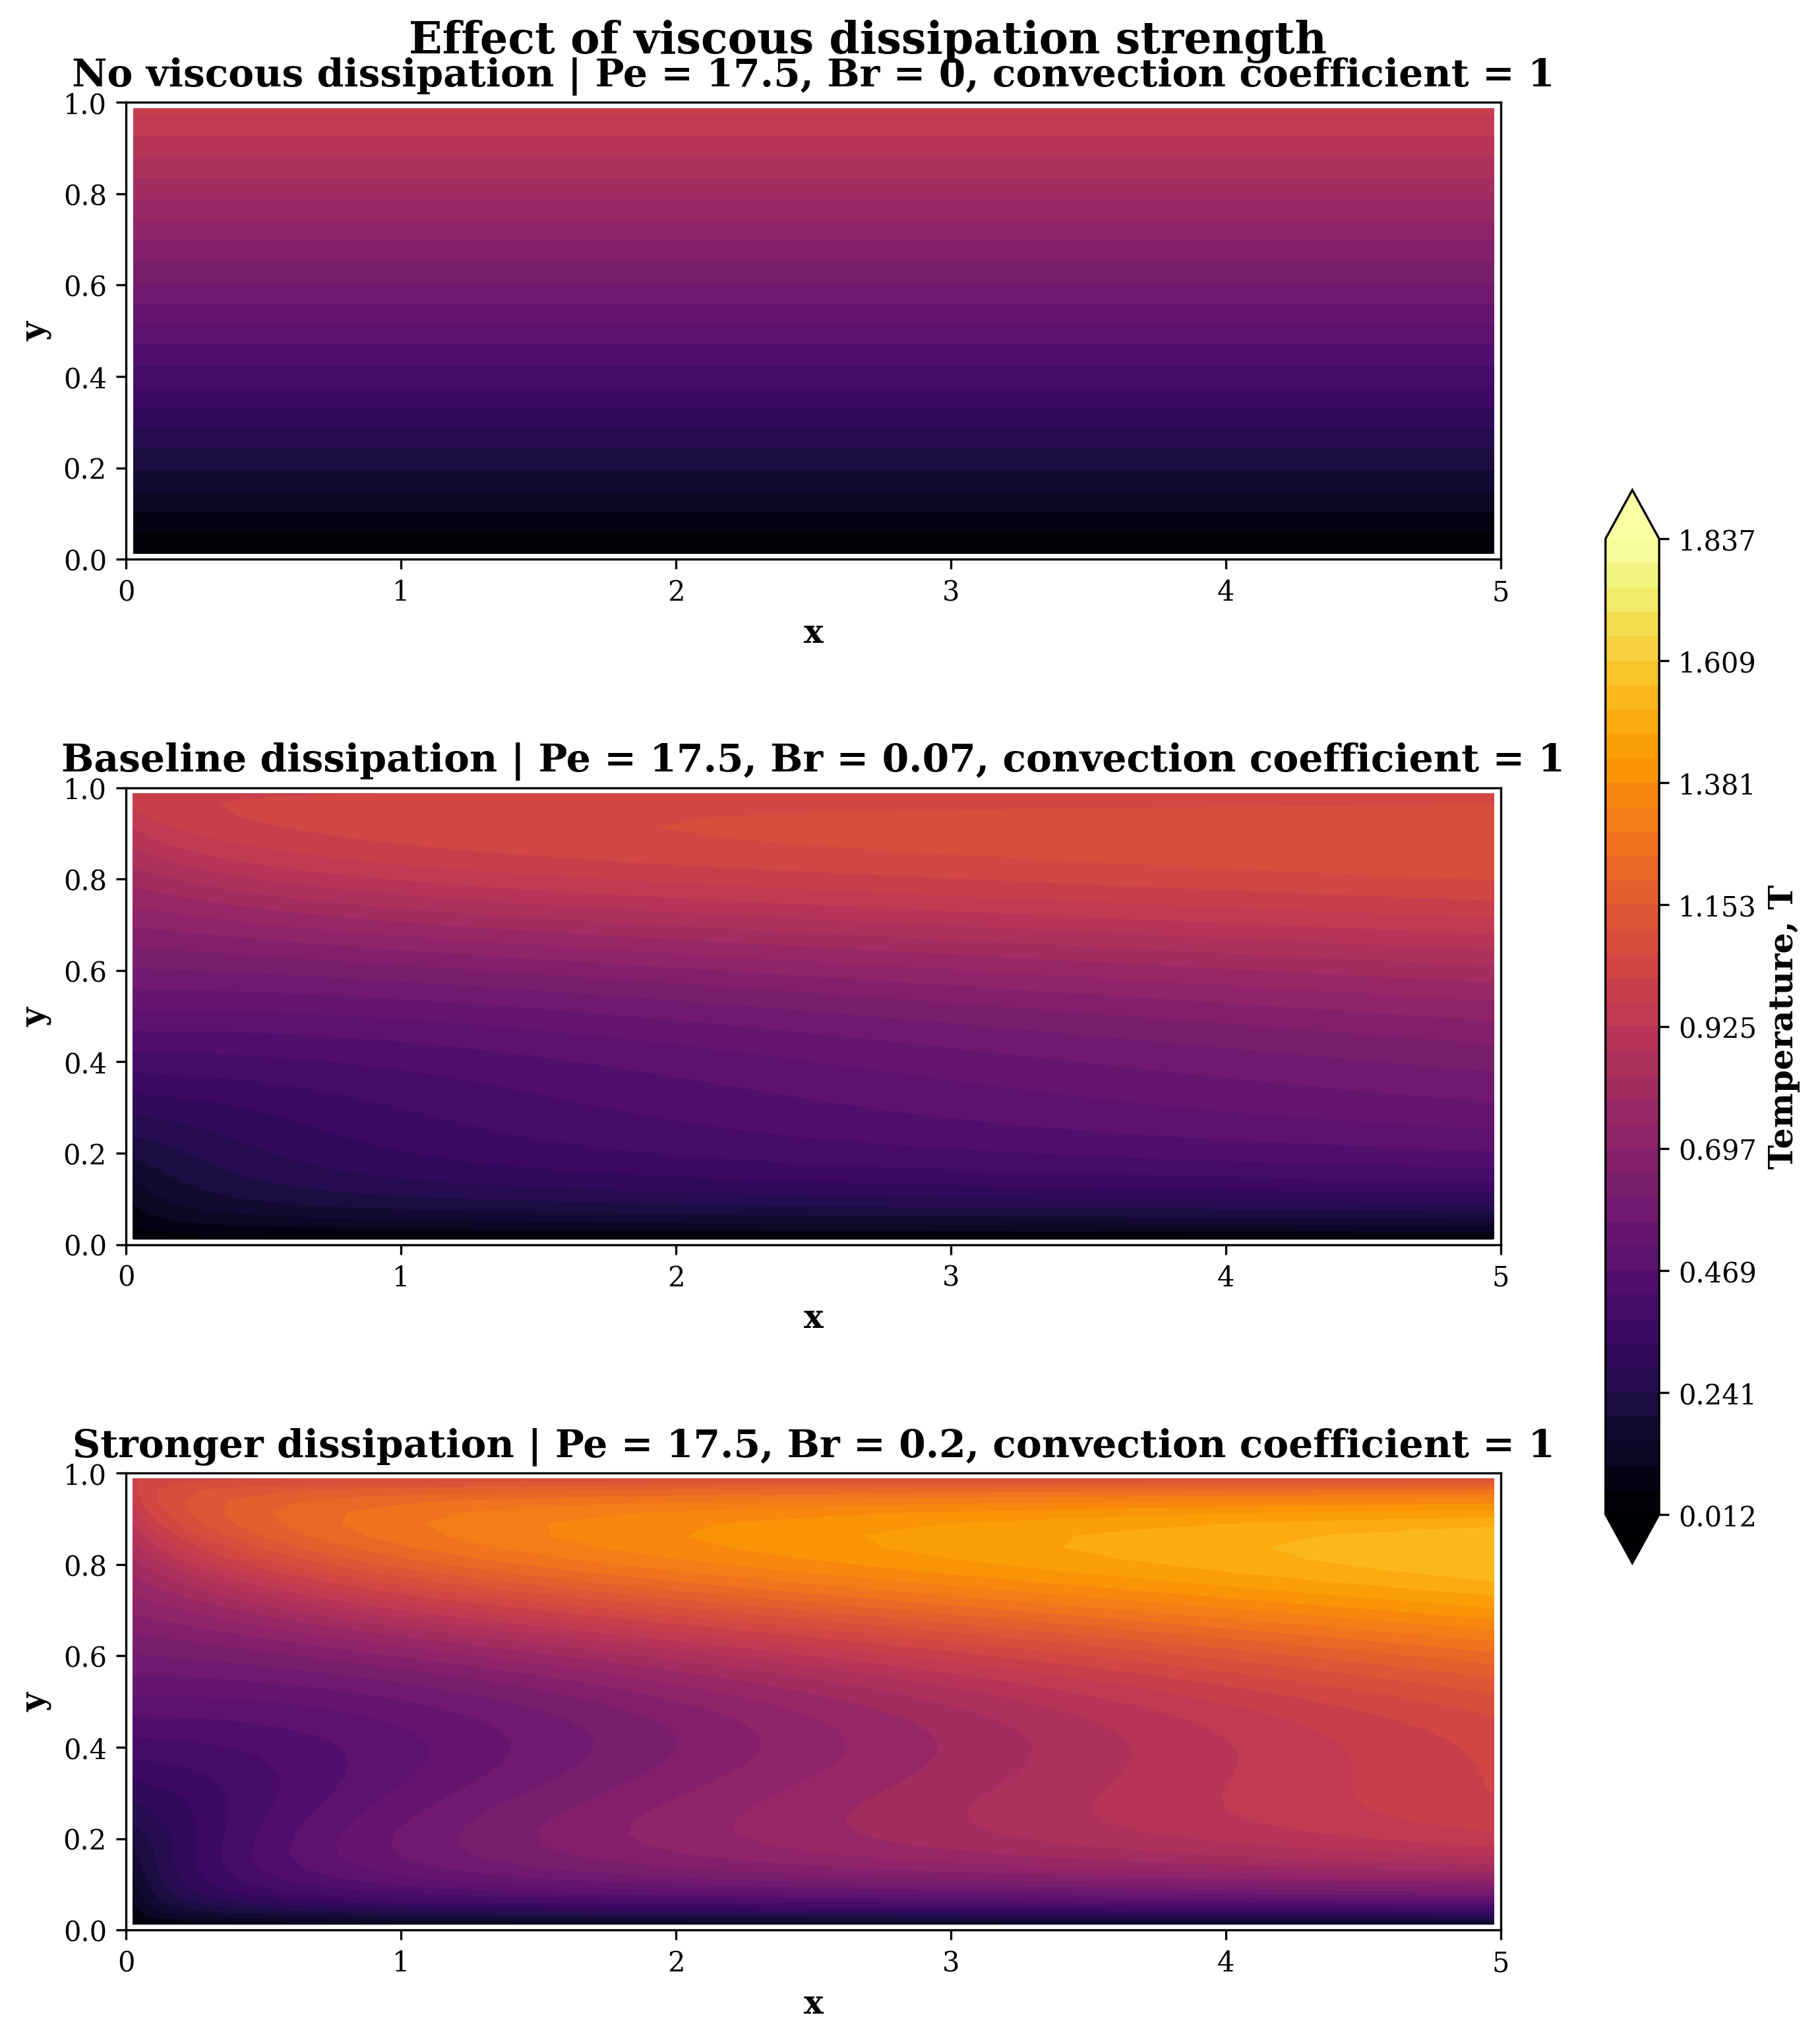
\includegraphics[width=0.88\textwidth]
    {figures/brinkman_number.png}
    \caption{Effect of the Brinkman number on the steady-state temperature
    distribution for $Pe=17.5$ and $\gamma_c=1$.}
    \label{fig:brinkman_study}
\end{figure}


\subsubsection{Effect of the Convection Coefficient}

The convection coefficient $\gamma_c$ scales the convective contribution
in the energy equation. Its effect was examined using
$\gamma_c=0.4$, $1$, and $10$, while keeping $Pe=17.5$ and $Br=0.2$
constant.

For a large convection coefficient, the temperature field remains closer
to the imposed inlet profile. This is expected because stronger convection
transports the inlet temperature distribution downstream and limits the
relative influence of thermal diffusion and viscous heating.

Reducing the convection coefficient weakens this transport. Consequently,
thermal diffusion and viscous dissipation have a greater influence on
the temperature field. The resulting distribution departs further from
the initial linear profile, with a more pronounced temperature increase
in the upper region of the channel.

The three cases are compared in Figure~\ref{fig:convection_study}.
The differences illustrate how the relative strengths of convection,
thermal diffusion, and viscous heating determine the resulting
temperature distribution.

\begin{figure}[htbp]
    \centering
    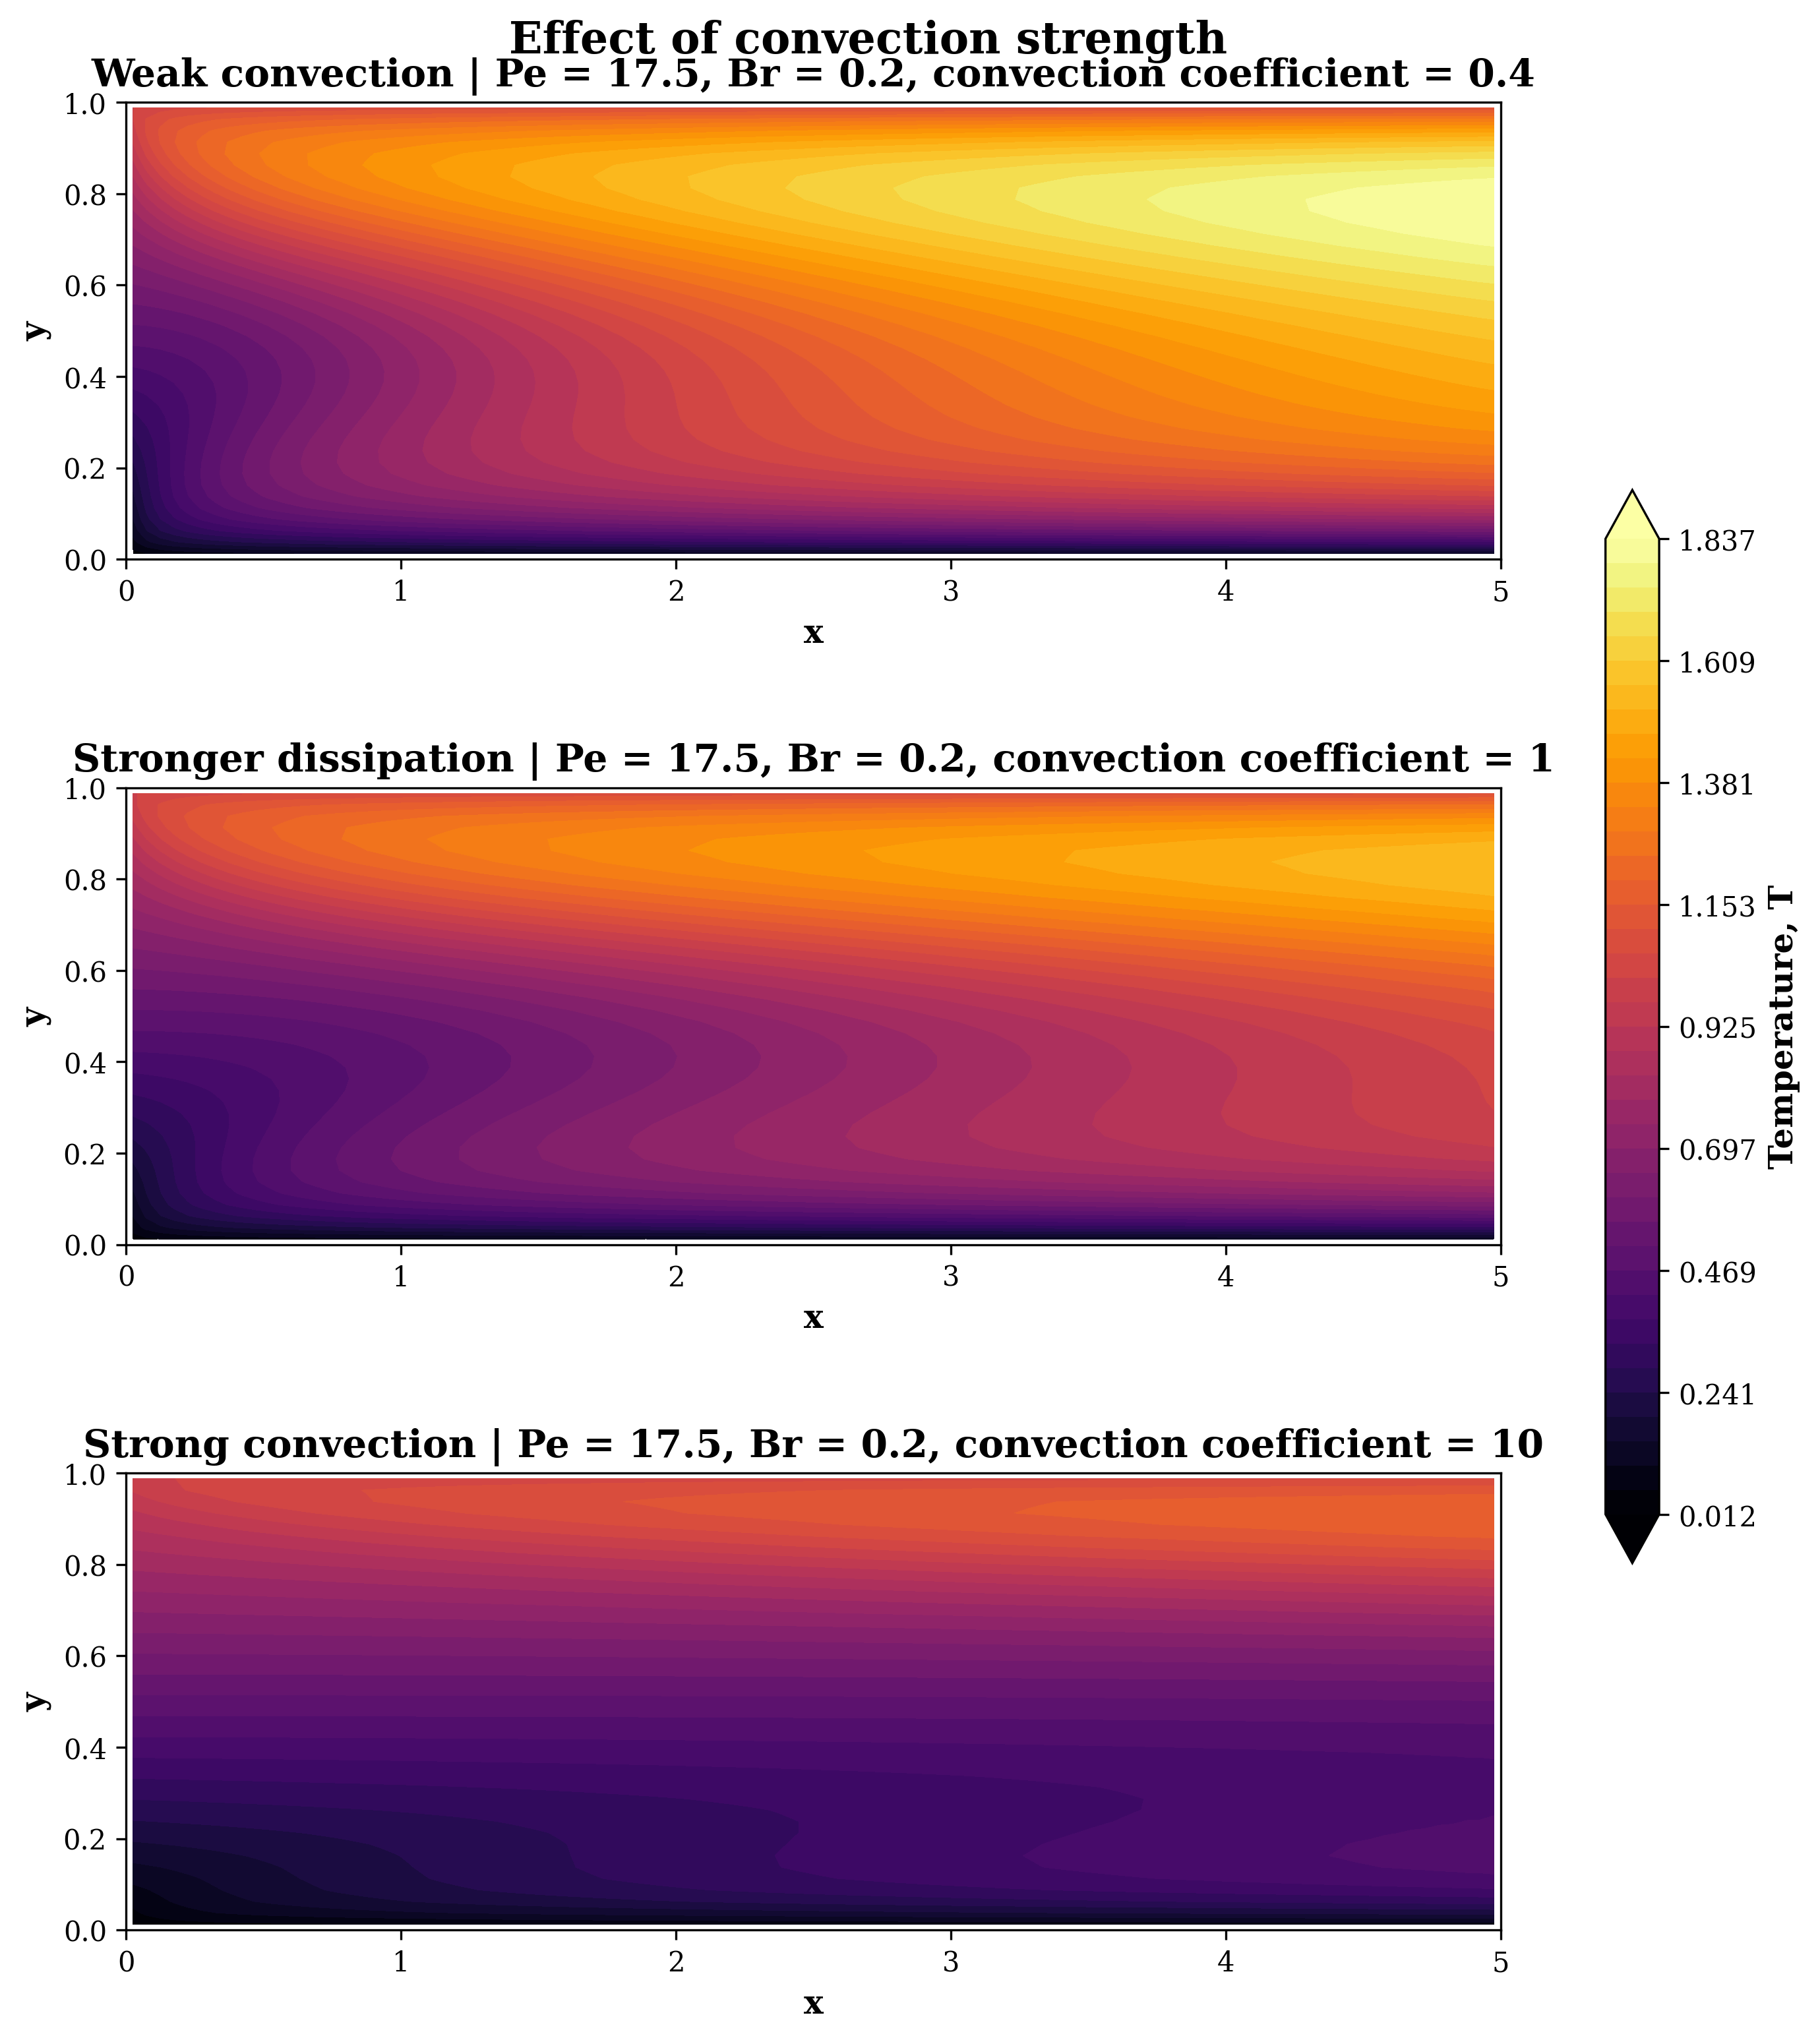
\includegraphics[width=0.88\textwidth]
    {figures/convection_coefficient.png}
    \caption{Effect of the convection coefficient on the steady-state
    temperature distribution for $Pe=17.5$ and $Br=0.2$.}
    \label{fig:convection_study}
\end{figure}


\subsubsection{Effect of the Peclet Number}

The Peclet number represents the relative strength of convective transport
to thermal diffusion. Its effect was studied at
$Pe=1$, $17.5$, and $50$. In these cases, the ratio $Br/Pe$ was held
constant at $0.004$, so the coefficient of the viscous dissipation source
remained unchanged.

A low Peclet number corresponds to stronger thermal diffusion relative
to convection. Since the initial and inlet temperature profiles are
identical, the temperature field tends to remain close to the linear
distribution. Thermal diffusion also smooths temperature variations
produced by the viscous heating source.

As the Peclet number increases, the relative influence of thermal
diffusion decreases. The temperature field therefore exhibits a greater
departure from the initial profile under the combined effects of
convection and viscous dissipation. In particular, the temperature
variations generated by the dissipation source are less strongly
smoothed by diffusion.

Figure~\ref{fig:peclet_study} compares the temperature fields at the
three Peclet numbers. The results demonstrate the influence of thermal
diffusion on the balance between convective transport and viscous
heating.

\begin{figure}[htbp]
    \centering
    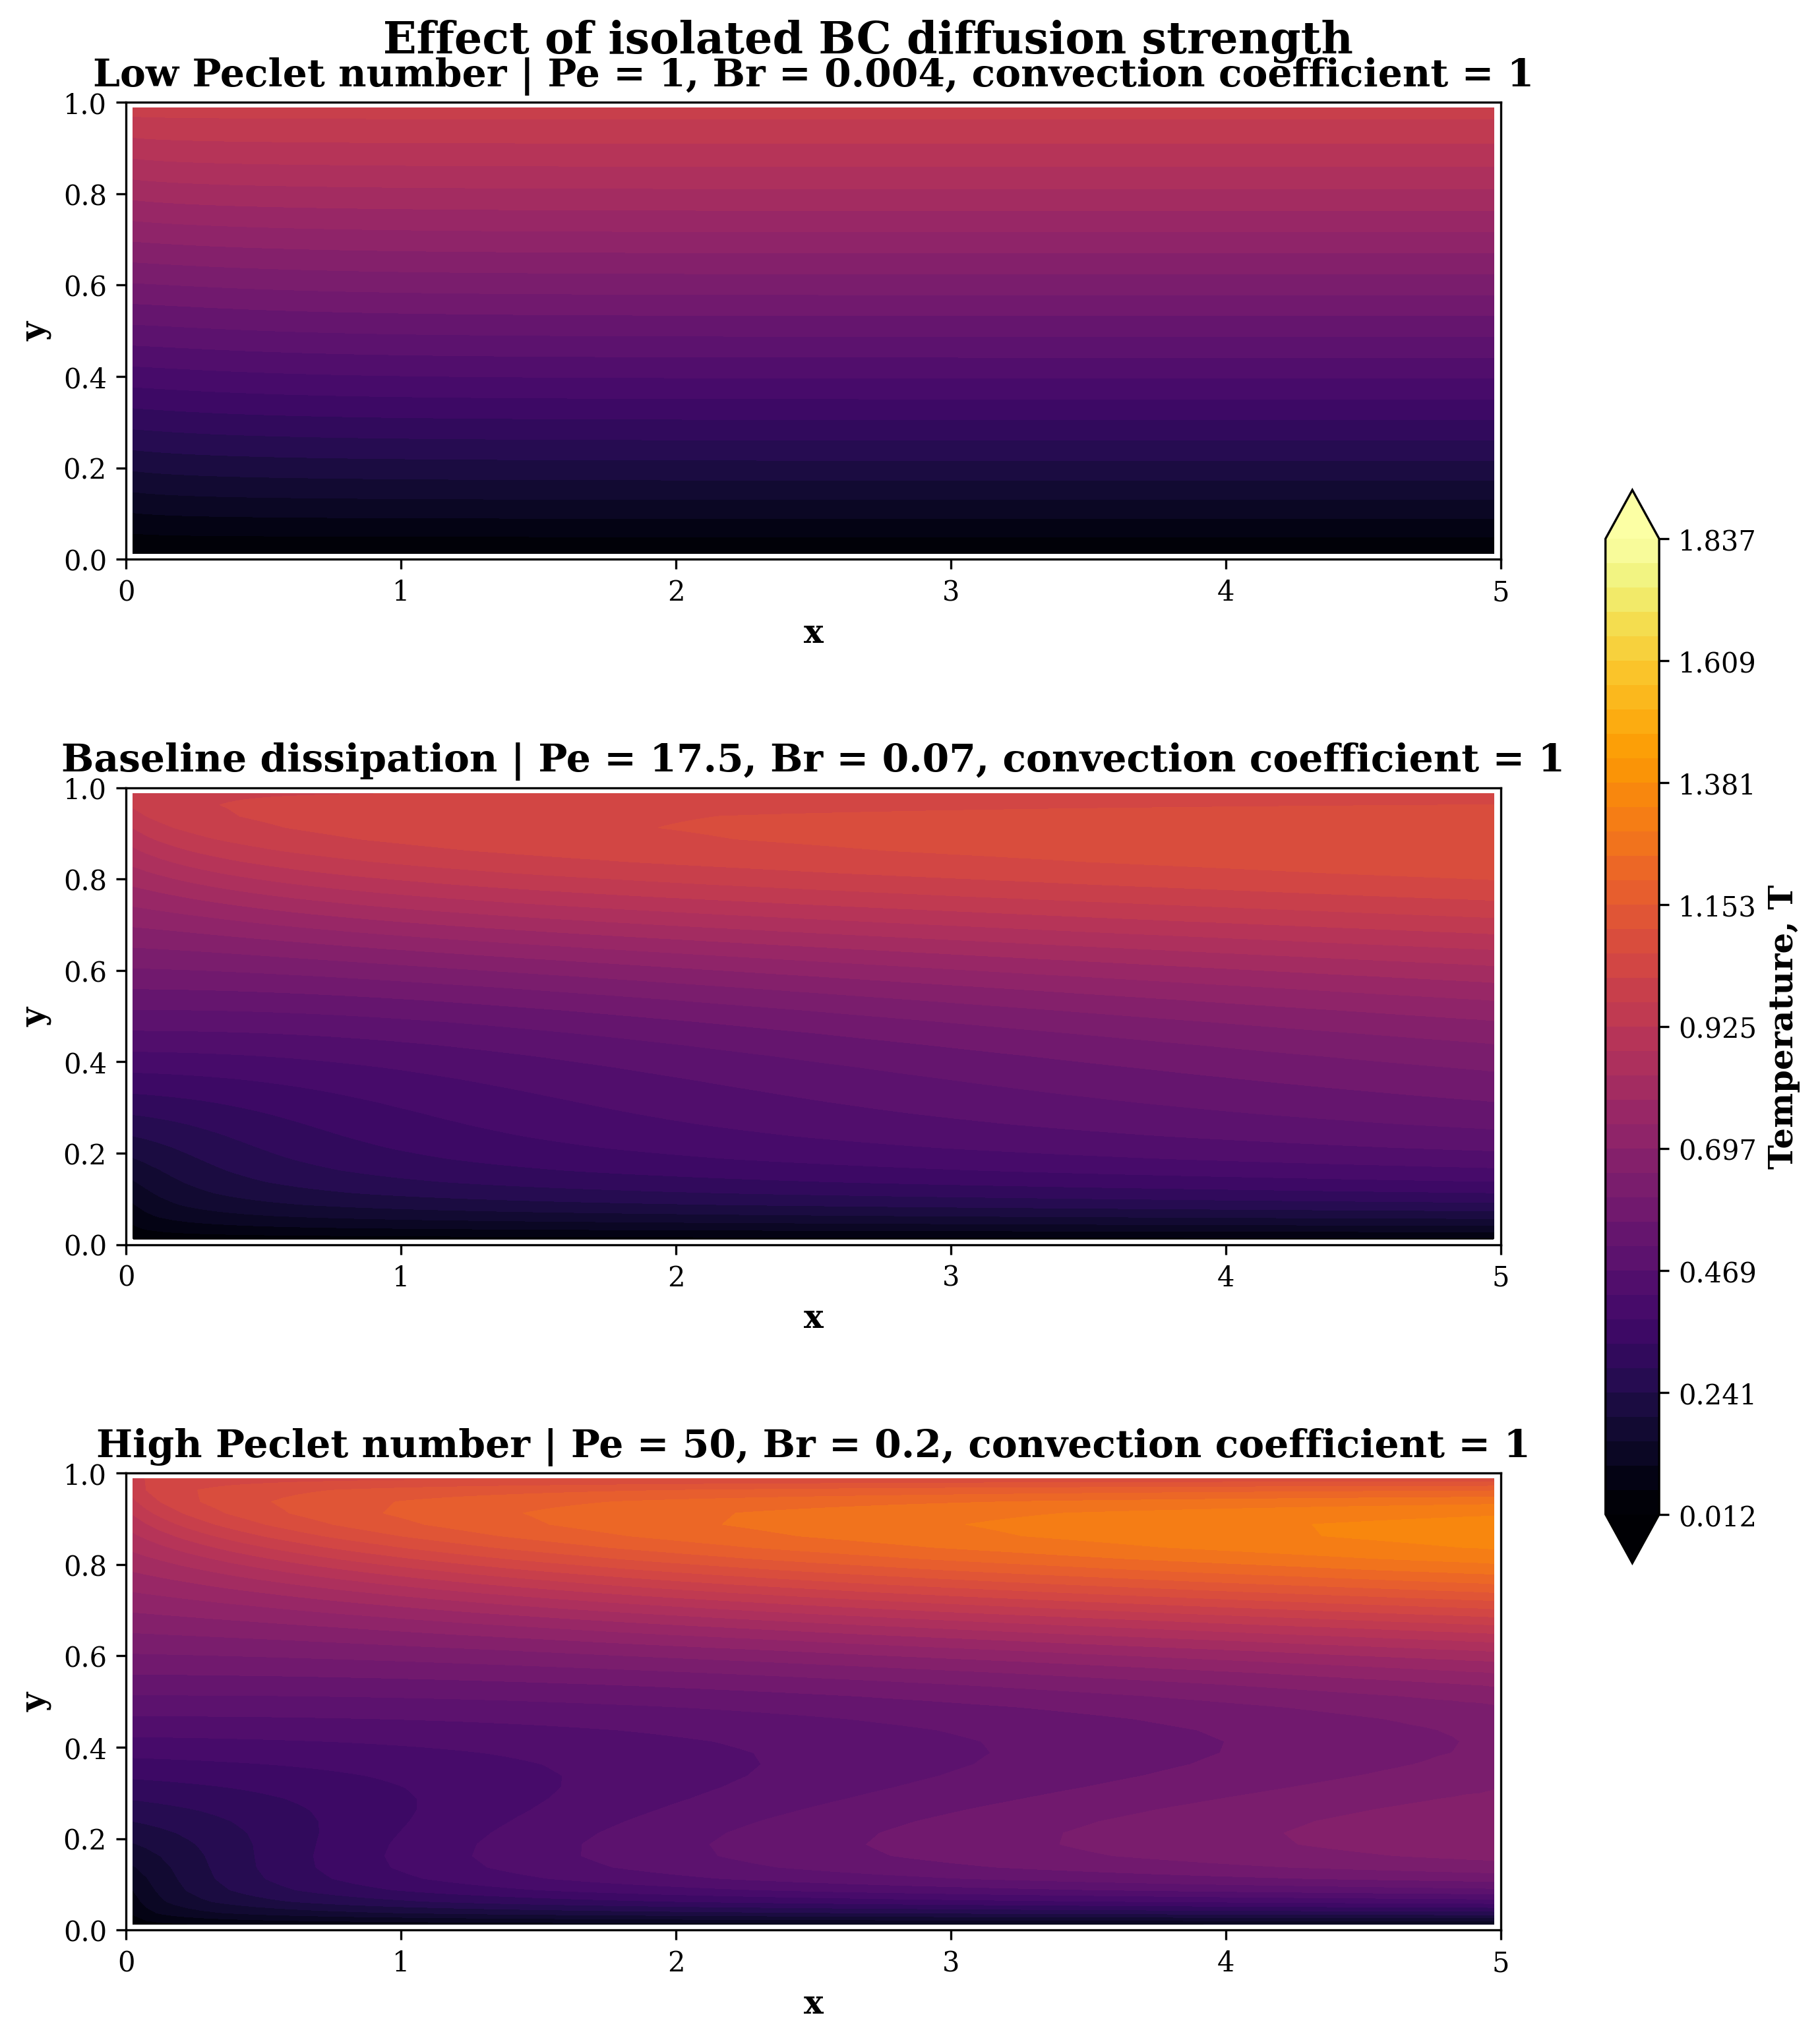
\includegraphics[width=0.88\textwidth]
    {figures/peclet_number.png}
    \caption{Effect of the Peclet number on the steady-state temperature
    distribution, with $Br/Pe=0.004$ and $\gamma_c=1$.}
    \label{fig:peclet_study}
\end{figure}


\subsubsection{Temperature Cross-Sections}

To examine the combined effects of convection and viscous dissipation
in more detail, temperature profiles were extracted at two streamwise
locations, $x/L_x=0.15$ and $0.85$. Three cases were selected for this
comparison:

\begin{itemize}
    \item Case 1: $Pe=17.5$, $Br=0.07$, and $\gamma_c=1$.
    \item Case 2: $Pe=17.5$, $Br=0.2$, and $\gamma_c=1$.
    \item Case 3: $Pe=17.5$, $Br=0.2$, and $\gamma_c=0.4$.
\end{itemize}

The first two cases have identical Peclet numbers and convection
coefficients. Their comparison therefore isolates the effect of
viscous dissipation. Increasing the Brinkman number from $0.07$ to
$0.2$ produces a more pronounced curvature in the wall-normal
temperature profiles. This reflects the stronger contribution of
viscous heating to the energy balance.

The second and third cases have the same Peclet and Brinkman numbers,
but different convection coefficients. Reducing $\gamma_c$ from
$1$ to $0.4$ weakens convective transport and increases the relative
influence of thermal diffusion and viscous heating. The resulting
profiles exhibit a warmer upper region and a less pronounced
wave-like variation, consistent with the smoothing effect of thermal
diffusion.

Together, these comparisons show that the temperature profiles result
from the combined effects of convective transport, thermal diffusion,
and viscous dissipation. Their relative contributions determine both
the temperature level and the shape of the wall-normal profiles.

\begin{figure}[htbp]
    \centering
    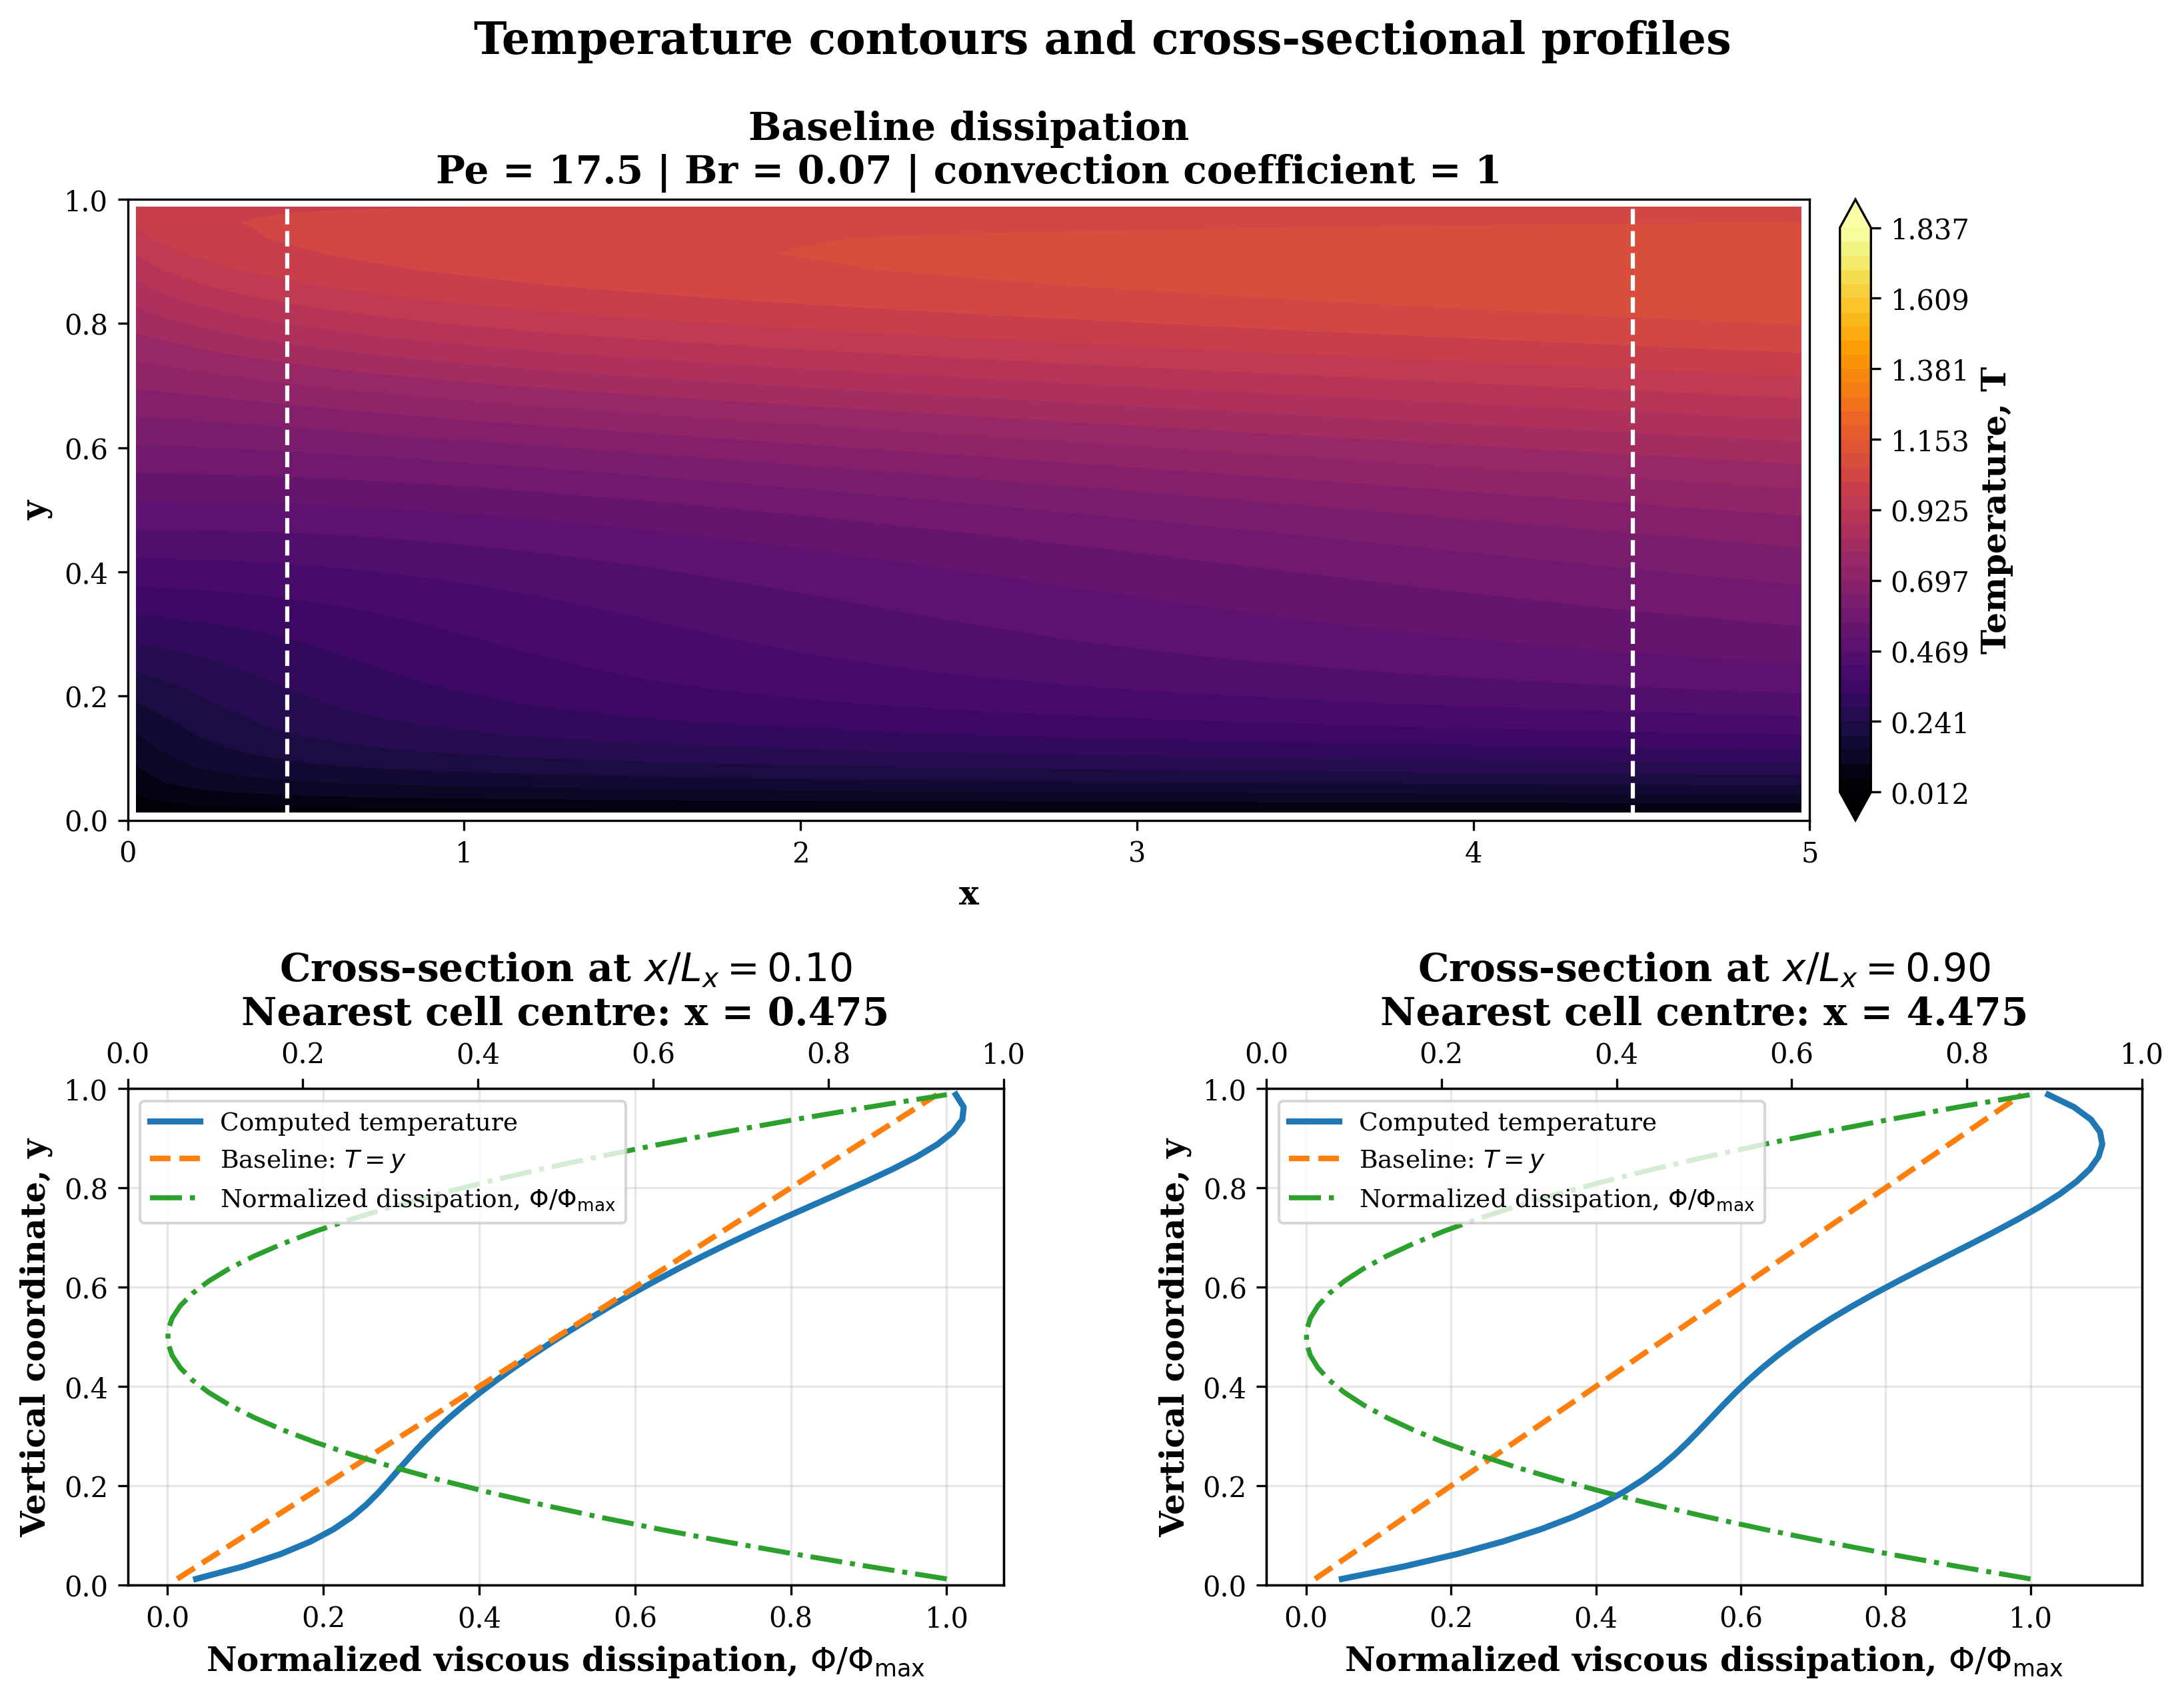
\includegraphics[width=0.88\textwidth]
    {figures/br_007_cross_sections.png}
    \caption{Temperature contours and wall-normal temperature profiles
    for $Pe=17.5$, $Br=0.07$, and $\gamma_c=1$.}
    \label{fig:cross_sections_br007}
\end{figure}

\begin{figure}[htbp]
    \centering
    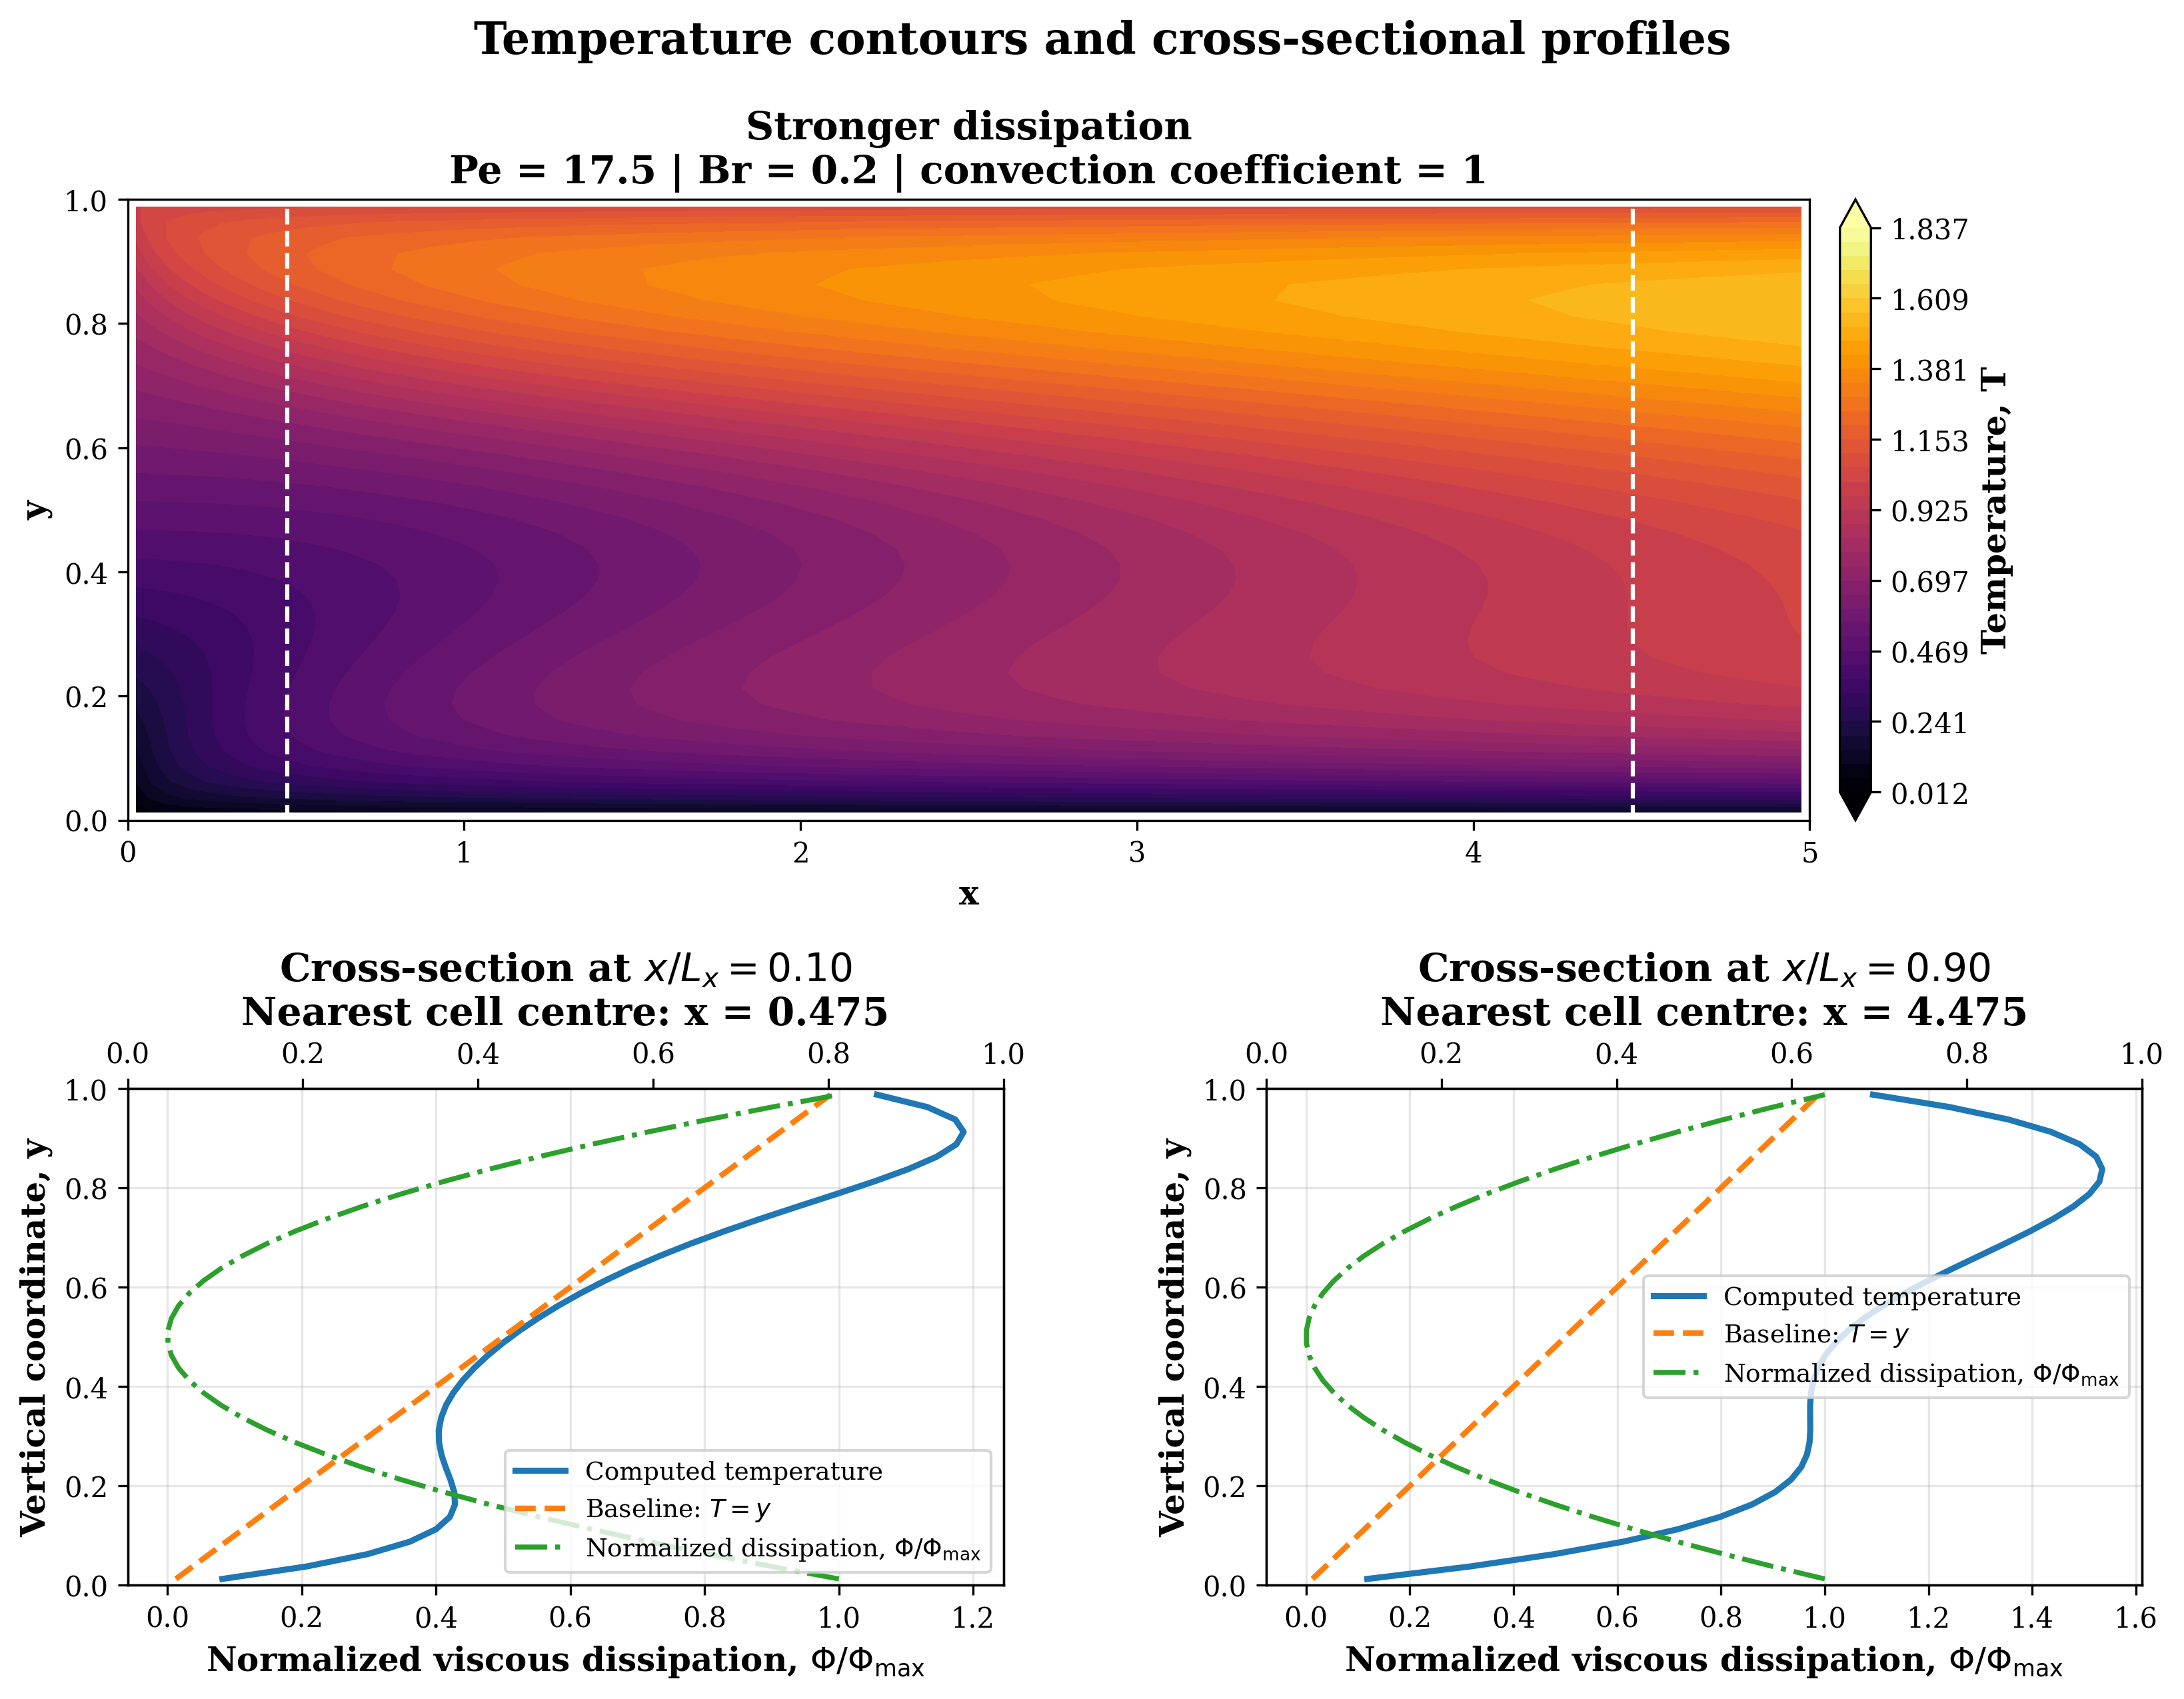
\includegraphics[width=0.88\textwidth]
    {figures/br_02_cross_sections.png}
    \caption{Temperature contours and wall-normal temperature profiles
    for $Pe=17.5$, $Br=0.2$, and $\gamma_c=1$.}
    \label{fig:cross_sections_br02}
\end{figure}

\begin{figure}[htbp]
    \centering
    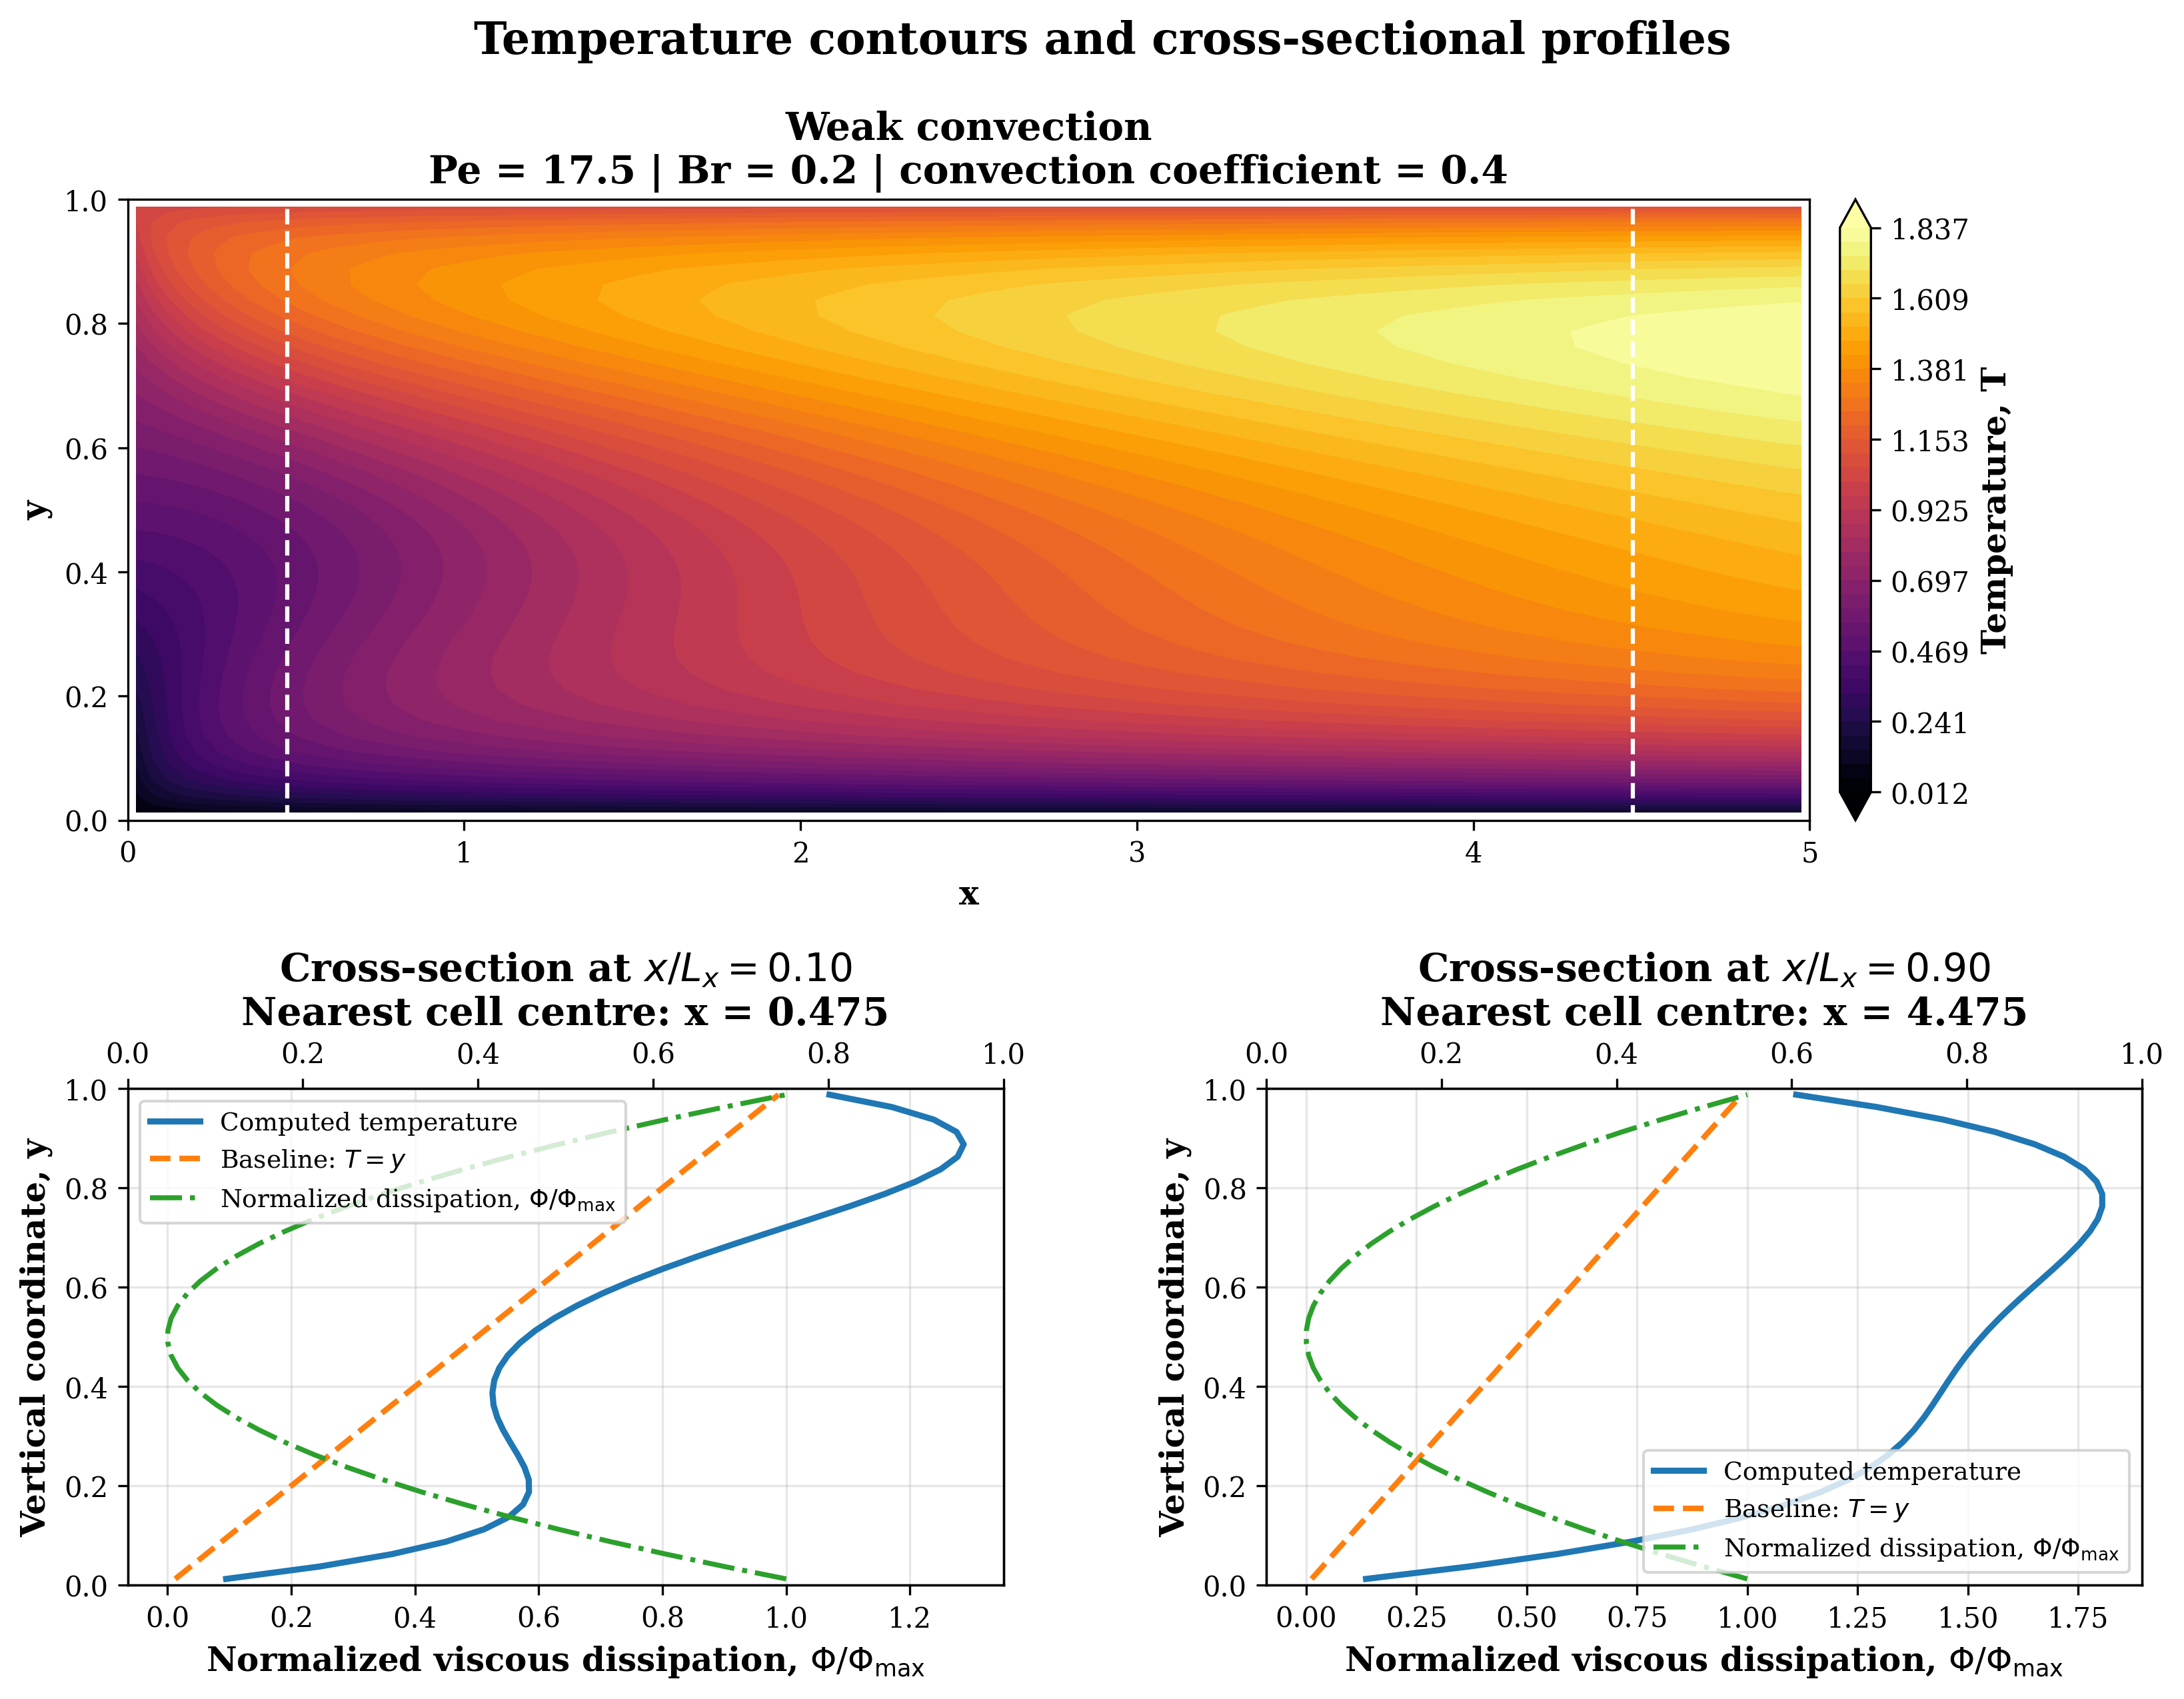
\includegraphics[width=0.88\textwidth]
    {figures/gamma_04_cross_sections.png}
    \caption{Temperature contours and wall-normal temperature profiles
    for $Pe=17.5$, $Br=0.2$, and $\gamma_c=0.4$.}
    \label{fig:cross_sections_gamma04}
\end{figure}